% Options for packages loaded elsewhere
\PassOptionsToPackage{unicode}{hyperref}
\PassOptionsToPackage{hyphens}{url}
%
\documentclass[
  12pt,
]{book}
\usepackage{amsmath,amssymb}
\usepackage{lmodern}
\usepackage{iftex}
\ifPDFTeX
  \usepackage[T1]{fontenc}
  \usepackage[utf8]{inputenc}
  \usepackage{textcomp} % provide euro and other symbols
\else % if luatex or xetex
  \usepackage{unicode-math}
  \defaultfontfeatures{Scale=MatchLowercase}
  \defaultfontfeatures[\rmfamily]{Ligatures=TeX,Scale=1}
  \setmainfont[]{Times New Roman}
\fi
% Use upquote if available, for straight quotes in verbatim environments
\IfFileExists{upquote.sty}{\usepackage{upquote}}{}
\IfFileExists{microtype.sty}{% use microtype if available
  \usepackage[]{microtype}
  \UseMicrotypeSet[protrusion]{basicmath} % disable protrusion for tt fonts
}{}
\makeatletter
\@ifundefined{KOMAClassName}{% if non-KOMA class
  \IfFileExists{parskip.sty}{%
    \usepackage{parskip}
  }{% else
    \setlength{\parindent}{0pt}
    \setlength{\parskip}{6pt plus 2pt minus 1pt}}
}{% if KOMA class
  \KOMAoptions{parskip=half}}
\makeatother
\usepackage{xcolor}
\IfFileExists{xurl.sty}{\usepackage{xurl}}{} % add URL line breaks if available
\IfFileExists{bookmark.sty}{\usepackage{bookmark}}{\usepackage{hyperref}}
\hypersetup{
  pdftitle={History of the Piedmont Neighborhood 1850-1920},
  pdfauthor={Jan de Leeuw},
  hidelinks,
  pdfcreator={LaTeX via pandoc}}
\urlstyle{same} % disable monospaced font for URLs
\usepackage{longtable,booktabs,array}
\usepackage{calc} % for calculating minipage widths
% Correct order of tables after \paragraph or \subparagraph
\usepackage{etoolbox}
\makeatletter
\patchcmd\longtable{\par}{\if@noskipsec\mbox{}\fi\par}{}{}
\makeatother
% Allow footnotes in longtable head/foot
\IfFileExists{footnotehyper.sty}{\usepackage{footnotehyper}}{\usepackage{footnote}}
\makesavenoteenv{longtable}
\usepackage{graphicx}
\makeatletter
\def\maxwidth{\ifdim\Gin@nat@width>\linewidth\linewidth\else\Gin@nat@width\fi}
\def\maxheight{\ifdim\Gin@nat@height>\textheight\textheight\else\Gin@nat@height\fi}
\makeatother
% Scale images if necessary, so that they will not overflow the page
% margins by default, and it is still possible to overwrite the defaults
% using explicit options in \includegraphics[width, height, ...]{}
\setkeys{Gin}{width=\maxwidth,height=\maxheight,keepaspectratio}
% Set default figure placement to htbp
\makeatletter
\def\fps@figure{htbp}
\makeatother
\setlength{\emergencystretch}{3em} % prevent overfull lines
\providecommand{\tightlist}{%
  \setlength{\itemsep}{0pt}\setlength{\parskip}{0pt}}
\setcounter{secnumdepth}{5}
\ifLuaTeX
  \usepackage{selnolig}  % disable illegal ligatures
\fi

\title{History of the Piedmont Neighborhood 1850-1920}
\author{Jan de Leeuw}
\date{Started in 2016. Last update August 31, 2021}

\begin{document}
\maketitle

{
\setcounter{tocdepth}{4}
\tableofcontents
}
\begin{figure}
\centering
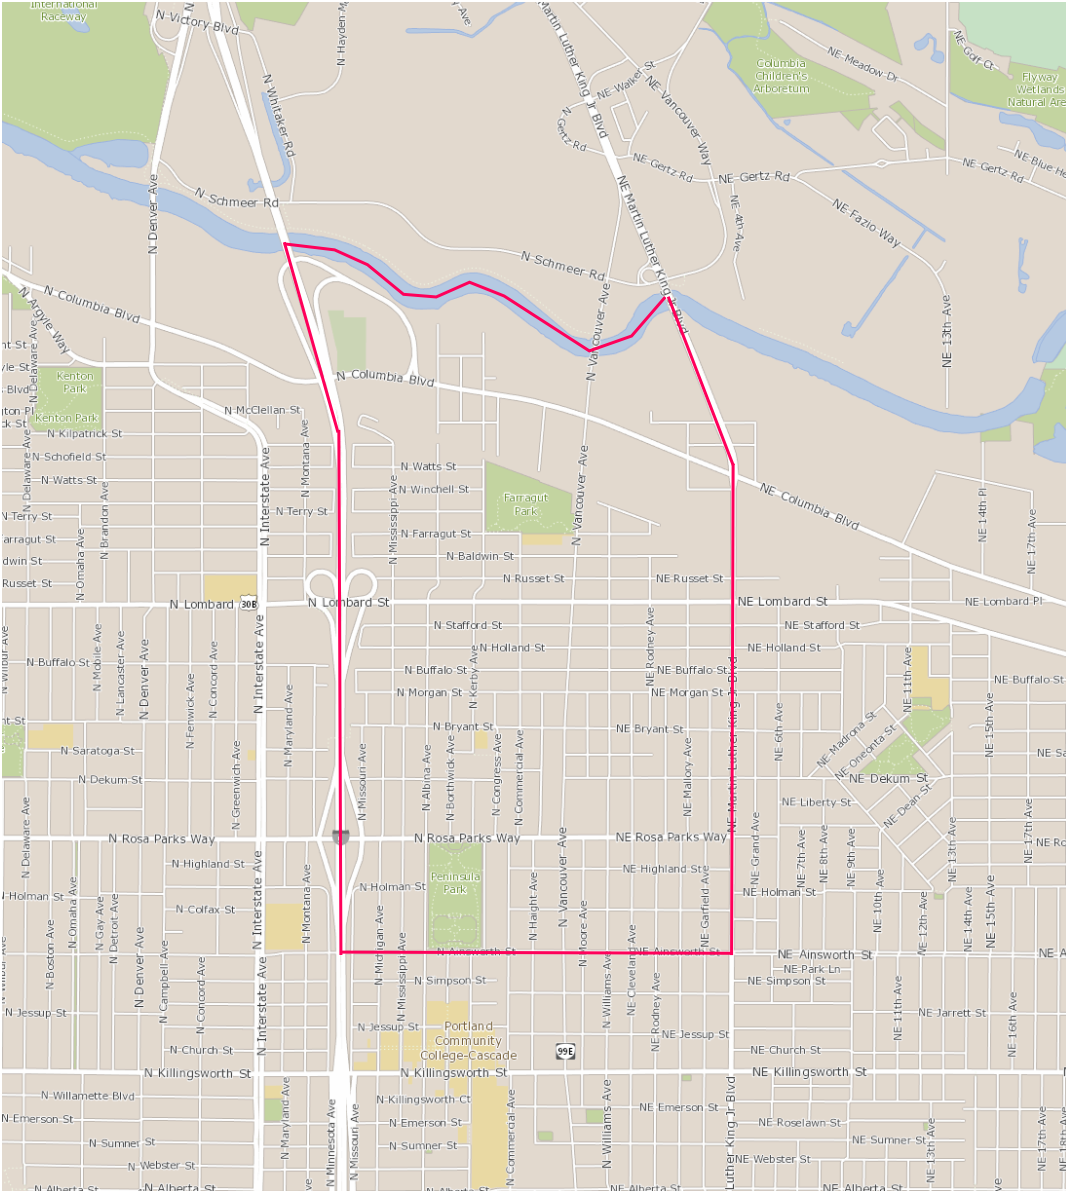
\includegraphics{images/00_images/image1.png}
\caption{alt\_text}
\end{figure}

\hypertarget{introduction}{%
\chapter*{Introduction}\label{introduction}}
\addcontentsline{toc}{chapter}{Introduction}

\hypertarget{piedmont}{%
\section*{Piedmont}\label{piedmont}}
\addcontentsline{toc}{section}{Piedmont}

Piedmont is one of the 95 neighborhoods in the neighborhood system of Portland, Oregon, and one of the eleven neighborhoods in the North Portland district coalition.

\begin{quote}
\emph{Portland's nationally recognized neighborhood system is made up of 95 recognized,
independent neighborhood associations and seven neighborhood district coalition offices
that represent the entire city of Portland.
\url{https://www.portlandoregon.gov/oni/28989}}
\end{quote}

The Piedmont neighborhood gets its name from the Piedmont subdivision, platted in 1889 by Edward Quackenbush and the Investment Company. And the Piedmont subdivision gets its name from the region in northwest Italy, known for its gentle slopes and hillsides. I am pretty sure the name Piedmont was chosen for its commercial appeal, and not for the physical resemblance with the eponymous region in Italy, which actually looks quite different.

Although:\url{https://en.wikipedia.org/wiki/Piedmont_(United_States)}

The Piedmont subdivision is only a small part of the Piedmont neighborhood, in fact less than ten percent of its area. And, conversely, only half of the Piedmont subdivision is in the Piedmont neighborhood, the rest is in Humboldt and King.

\hypertarget{land}{%
\section{Land}\label{land}}

Throughout this book, I concentrate on land and land ownership. It is essential, therefore, to remember that Oregon, Portland, and Piedmont were started by settler colonialism. This meant the United States occupied lands used for centuries by indigenous peoples, and declared it to be public lands of the United States. War, terror, vigilantes, disease, broken treaties, racism, religion, and unjust laws made sure the unceded lands stayed in the hands of the occupying forces. The small percentage of indigenous people that survived the onslaught were driven onto ever shrinking reservations. In the middle of the nineteenth century, when settlers started to arrive and Portland became a fast growing city, there were very few Native Americans left in the area.

In that nineteenth century the United States adopted laws which encouraged settlement by giving large sections of public lands away (usually tracts of 160 acres), and making other sections available for very little money (usually for \$ 1.25 per acre). The land that currently makes up Piedmont was donated in this way to just four people. Evander Howe, George Smith, Lewis Love, and David Ulery were all farmers on the Vancouver Road, near the Columbia Slough. They could effectively use the Donation Land Claim Act and the Military Bounty Law, because they were the first settlers to arrive, and actually for quite some time the only settlers to arrive.

In the next stage the city grew because the settlers, or ``pioneers'', sold their land to developers, who platted subdivisions. Piedmont over the years became differentiated from about four homesteads to about 30 subdivisions of varying sizes. From 1850 on fortunes were made by subdividing, exchanging, transfering, inheriting, buying, and selling pieces of land. In the third stage of development each of the subdivisions, sometimes also called additions, were partitioned into a varying number of city blocks, usually 200 by 200 feet, and the blocks were partitioned in lots, usually eight lots of 100 by 50 feet. These individual lots were then sold to people to build their houses, or packaged into multiple lots for speculation. Piedmont consists of thousands of such lots.

In the book I will discuss the original homesteads and the subsequent subdivisions. As a consequence of this emphasis on land, the book concentrates on the time between 1850 and 1930. After 1930 development is mostly down to the level of individual lots, and since there are about 5000 of these, I cannot discuss them one by one. It is interesting, of course, to find out who built an individual house, and who the subsequent owners were. But the sheer number of them makes it impossible to write about each and every one.

\hypertarget{bias}{%
\section{Bias}\label{bias}}

As you will probably figure out quickly, I like maps. I also like facts, more than I like opinions. I like words, more than I like photographs. Thus this book is not of the coffee table type, with many photos and only a few words.

I also do not like the view that historical developments are driven by a small number of important individuals, always men of course, and that we want to know as much as possible about these men, possibly because we want to become just like them. History is driven by social and economic forces and movements in which specific individuals are of limited and largely anecdotal significance. I like to report about structures and systems more than I like to report about people. Also, I hope that what I do report about the men and women that were important in Piedmont's early history makes it clear that you do not necessarily want to become just like them.

There are two other important types of Portland history books I do not want to emulate. Some of them are excellent, but they are not what I am interested in. There are those books that concentrate on vice, corruption, crime, shanghaiing, and prostitution. They are mostly about the northwest of Portland, between 1870 and 1910. And then there are those books that tell the story of city government and the business community, again mostly although not entirely about the part of Portland west of the river. As far as I am concerned, these two types of books talk about two sides of the same coin, a bunch of people quibbling on how to divide the loot. Of course that describes a huge part of history in general, and in this book the loot is basically two square miles of land, sections 10 and 15 in township one north, range one east of the Willamette Meridian.

\hypertarget{technical}{%
\section{Technical}\label{technical}}

This book is, and always will be, free and in the public domain. Anyone can copy, print, distribute or otherwise use the material in this book for any purpose whatsoever, and, if they so choose, without attribution.

All references are collected in the back of each chapter or section. I have tried to make everything reproducible, in the sense that every statement of fact that I make can be traced back to its sources. I have also tried to emphasize primary (i.e.~contemporaneous) sources, even if they were only newspaper articles. Secondary sources are only used, reluctantly, if primary sources are not available. I have also tried to refrain, as much as is humanly possible, from stating opinions about events, or making inferences about motives.

This book is a living document, which means that any part of it can change at any moment. Thus all sections have a date attached to their title, indicating when they were last changed. I keep discovering new facts and adding new materials. In the table of contents each section is linked to a separate pdf, which is synchronized with the sections in the Google docs version of the book.

This book is also, among other things, a repository. There are copies of, or links to, the original maps, deeds, photos, and newspaper articles that the narrative is based on. If you see a link below a figure or a map, then following that link will usually get you to a bigger and better version of the map you can either download to your computer or view in your browser. Generally you get the best resolution by downloading the file and opening it in the appropriate application.

\hypertarget{references}{%
\section{References}\label{references}}

The City of Portland, Oregon. \emph{Neighborhood Program.}
\url{https://www.portlandoregon.gov/oni/28989}

Alta Mitchoff: \emph{History of the Kenton Neighborhood}
Kenton Neighborhood Association, 1997

Anjala Ehelebe:\_ Portland's Woodlawn Neighborhood\_
Arcadia Publishing, 2008

Roy E. Roos: \emph{The History and Development of Portland's Irvington Neighborhood}
Self published, 1997

Roy E. Roos: \emph{The History of Albina. Including Eliot, Boise, King, Humboldt, and Piedmont Neighborhoods.}
Self published, 2008

\hypertarget{they-were-here-first.-and-they-are-still-here.}{%
\chapter{They Were Here First. And They Are Still Here.}\label{they-were-here-first.-and-they-are-still-here.}}

\begin{figure}
\centering
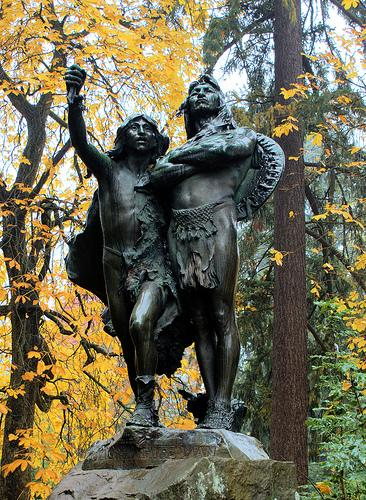
\includegraphics{images/01_images/image1.jpg}
\caption{alt\_text}
\end{figure}

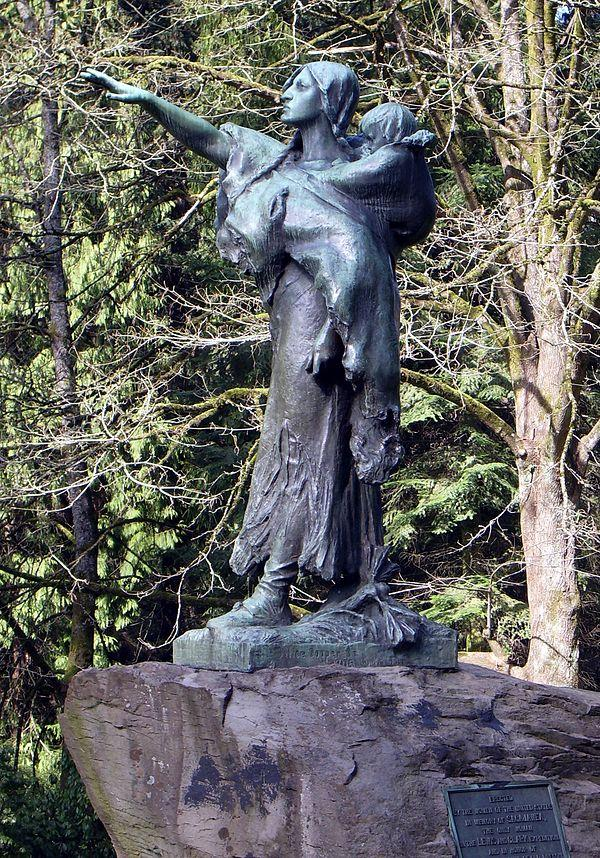
\includegraphics{images/01_images/image2.jpg}
\#\# Introduction

They made us many promises, more than I can remember.

But they kept only one -- They promised to take our land \ldots{} and they took it.

Red Cloud, Lakota, around 1900

It is appropriate to start this book with a chapter on the Native Americans who were here first and who lived on the land that is currently the Piedmont Neighborhood. It turns out that this is far from easy. I will have to rely heavily on a huge amount of research on relatively sparse data, documented most thoroughly in an excellent recent edited volume.

Robert T. Boyd, Kenneth M. Ames, Tony A. Johnson (eds): \emph{Chinookan Peoples of the Lower Columbia.} University of Washington Press, 2013.

To set the scene we start with two statues in Washington Park. The first one, on the left, is called ``\emph{The Coming of the White Man}''. The sculptor was Hermon Atkins MacNeil (1866 -- 1947), who specialized in Native American scenes. This particular statue was gifted to the City of Portland in 1904 by former mayor \href{https://en.wikipedia.org/wiki/David_P._Thompson}{David P. Thompson}. It depicts two Native American men looking towards the \href{https://en.wikipedia.org/wiki/Columbia_River}{Columbia River} upon the arrival of \href{https://en.wikipedia.org/wiki/Lewis_and_Clark_Expedition}{Lewis and Clark}. The older man, with arms crossed, is supposedly Chief Multnomah, the younger one is not identified. Sculptor MacNeil continued to make and sell many separate copies of the Chief Multnomah figure.

There are some problems with the statue, independent of its artistic merits. First, there is a relatively minor historical problem. For a long time historians have denied that Chief Multnomah was an actual historical figure. Recent research (Fulton, 2005), relying on the native american oral tradition, maintains that he did indeed exist. He was a powerful and important chief, who controlled a large territory around the Willamette river, and commanded many warriors. He died around 1780, possibly in the first smallpox epidemic. Whether he existed or not, he was no longer living when Lewis and Clark arrived in 1804-1805.

The second problem, which was unavoidable at the time, is that the statue is firmly in the white supremacist tradition of the Noble Savage, the Theatrical Savage, and the Picturesque Savage (Ellington, 2001). A good way to illustrate this is with a contemporary review of the statue by one Arno Dosch in the Pacific Monthly of 1905.

\begin{verbatim}
_Mr. MacNeil has put thought and genius into that old chief. He has depicted a patriarch in the full possession of his bodily strength, with a frame of iron, legs of steel cords and an arm of certain stroke. He stand on his toes to see better, binding his knees with tendons and drawing the cords over his thighs, hollowing the hips and bringing out the groin line clear. His are the legs of perfect strength, with the veins showing a little more prominently than in a younger man. On an upright body, with arms folded and a shield slung over the back, rises the head. In the face is the power. It is that of a Multnomah, a man of mental ability, a brooding savage, an Indian chief. He guided his own people by his wisdom, and let them in conquest on the enemy. The neck is drawn in heavy cords, and upon it is the chin of hauteur, almost disdain, the eyes expectant, but not astonished; the nose masterful, the strong hair bound back by a band._
\end{verbatim}

The younger person is also described by Dosch.

\begin{verbatim}
_His attitude is in direct contrast to that of his elder. His whole body and face expresses open curiosity and wonderment. He holds aloft on his right hand a branch, just broken from a tree, and waves it as a token of good will to the strangers._
\end{verbatim}

At some point in time in the 1930's someone, presumably someone with a more keen sense of history, broke off this olive branch from the statue. It has not been restored.

Remember that Arno Dosch wrote in 1905. In the preceding 100 years an estimated ninety percent of the Native American population had disappeared. They largely succumbed to diseases brought by the white man. But they had also been hunted down and killed by vigilantes and slaughtered in staged so-called ``Indian Wars'' by the army. They were driven from their lands, tricked into signing treaties that would never be ratified, and they were forcibly removed to areas east of the Cascades, or driven onto small reservations of land that the white settlers did not want. In 1905 the expression on the face of Chief Multnomah should have alternated between immense sadness and equally immense rage.

The second statue in Washington Park, the picture on the right, is ``\emph{Sacajawea and Jean-Baptiste}''. The sculpture was commissioned for the \href{https://en.wikipedia.org/wiki/Lewis_and_Clark_Centennial_Exposition}{Lewis and Clark Centennial Exposition} (1905) by the Committee of Portland Women, who requested a sculpture of ``\emph{the only woman in the Lewis and Clark Expedition and in honor of the pioneer mother of old Oregon}.''

\hypertarget{before-contact}{%
\section{Before Contact}\label{before-contact}}

Archeology

\hypertarget{discovering-the-columbia}{%
\section{Discovering the Columbia}\label{discovering-the-columbia}}

\hypertarget{the-lewis-and-clark-journals}{%
\section{The Lewis and Clark Journals}\label{the-lewis-and-clark-journals}}

The two visits to Native American sites in the Columbia Basin/Wapato Valley

\hypertarget{the-wapato-valley-native-americans}{%
\section{The Wapato Valley Native Americans}\label{the-wapato-valley-native-americans}}

\hypertarget{the-spirit-of-pestilence}{%
\section{The Spirit of Pestilence}\label{the-spirit-of-pestilence}}

\hypertarget{the-extinction-of-indian-title}{%
\section{The Extinction of Indian Title}\label{the-extinction-of-indian-title}}

How the lands were taken away (In the Courts of the Conqueror, Conquest by Law).

\begin{verbatim}
_There has been some discussion as to the origin of our title to what was known as the Oregon country, comprising the State of Oregon, Washington and Idaho, and the portions of Montana and Wyoming west of the Rocky Mountains. The question wa whether our title was derived from the Louisiana Purchase or directly by discovery and prior possession. As the result of discussion by the General Land Office in 1898, the map of the United States now issued by that office states that the title was established in 1846. The exact basis of our claim has apparently never been authoritatively decided (Bien, 1910, page 388)._
\end{verbatim}

\hypertarget{present-day-multnomah-county}{%
\section{Present Day Multnomah County}\label{present-day-multnomah-county}}

\hypertarget{references-1}{%
\section{References}\label{references-1}}

Morris Bien: \emph{The Public Lands of the United States.}
The North American Review, 192, 1910, 387-402
\url{https://drive.google.com/file/d/1TT_lgoh_nI8LSdztGw_claFQYfHje16G}

Jerry A. O'Callaghan: \emph{The Disposition of the Public Domain in Oregon}
Dissertation submitted to the Department of History and the Committee on Graduate Study of Stanford University, November 1960
\url{https://drive.google.com/file/d/1T8HRj39qobQ_4NkydJpagwnRQvFPAEUB}

Gary E. Moulton (ed): \_The Lewis and Clark Journals. An American Epic of Discovery. The Abridgment of the Definitive Nebraska Edition. \_University of Nebraska Press, 2004

Gary E. Moulton (ed): \_The Definitive Journals of Lewis \& Clark. Down the Columbia to Fort Clatsop. \_Volume 6 of the Nebraska Edition. University of Nebraska Press, 1990.

Gary E. Moulton (ed): \_The Definitive Journals of Lewis \& Clark. From the Pacific to the Rockies. \_Volume 7 of the Nebraska Edition. University of Nebraska Press, 1991.

Robert T. Boyd, Kenneth M. Ames, Tony A. Johnson (eds): \emph{Chinookan Peoples of the Lower Columbia.} University of Washington Press, 2013.

Michael Silverstein: \_Chinookians of the Lower Columbia. \_In Wayne Suttles (ed): \emph{Handbook of North American Indians, Volume 7, Northwest Coast}, p 533-546. Washington, Smithsonian, 1990.

Robert H. Ruby and John A. Brown: \_The Chinook Indians. Traders of the Lower Columbia River. \_University of Oklahoma Press, Norman, Oklahoma, 1976.

Robert H. Ruby, John A. Brown, Cary C. Collins: \emph{A Guide to the Indian Tribes of the Pacific Northwest.} University of Oklahoma Press, Norman, Oklahoma, Third Edition, 2010.

Ann Curry-Stevens, Amanda Cross-Hemmer, Coalition of Communities of Color:\_ The Native American Community in Multnomah County. An Unsettling Profile. \_Portland State University, School of Social Work, 2011. \url{https://pdxscholar.library.pdx.edu/cgi/viewcontent.cgi?article=1093\&context=socwork_fac}

Robert A. Williams, Jr: \emph{The American Indian in Western Legal Thought.} \_The Discourses of Conquest. \_Oxford University Press, 1990

Robert A. Williams, Jr: \emph{Savage Anxieties.} \_The Invention of Western Civilization. \_Palgrave McMillan, 2012

Ann Fulton: \_The Restoration of Iłkák'mana: A Chief Called Multnomah. \_American Indian Quarterly, 31, 2007, 110-128

Ter Ellington: \emph{The Myth of the Noble Savage}. University of California Press, 2001.

Lindsay G. Robertson: \_Conquest by Law. How the Discovery of America Dispossessed Indigenous People of their Lands. \_Oxford University Press, 2005

Walter R. Echo-Hawk: \_In the Courts of the Conqueror. The 10 Worst Indian Law Cases Ever Decided. \_Fulcrum Publishing, 2012.

Arno Dosch: \_The Coming of the White Man. \_The Pacific Monthly, 13, 1905, 50-52

The Native American Community in Multnomah County:

\hypertarget{homesteaders-and-homesteads-introduction}{%
\chapter{Homesteaders and Homesteads: Introduction}\label{homesteaders-and-homesteads-introduction}}

\begin{figure}
\centering
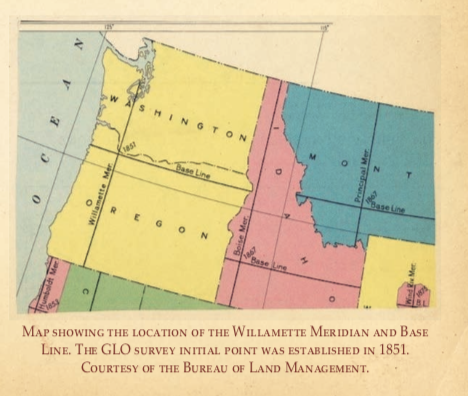
\includegraphics{images/02_images/image1.png}
\caption{alt\_text}
\end{figure}

\hypertarget{the-map}{%
\section{The Map}\label{the-map}}

The map above shows those donation lands and homesteads the United States handed out and sold around 1850-1860 that cover the Piedmont neighborhood (which is the area within the red boundaries). There is only a small number of them, five or so, and the large parcels (in the blue lines) in most cases also overlap with the adjacent neighborhoods Woodlawn, Overlook, Humboldt, King, Arbor Lodge, Kenton, and East Columbia. I shall use the generic name ``homesteads'' for these properties, although not all of them were authorized by the homestead act, and not all the original grantees actually homesteaded on them.

To put this in a larger context, here is the map of the 1860 survey of all of Township 1 of Range 1 east, which covers all of Portland, including East Portland and Albina.

\begin{figure}
\centering
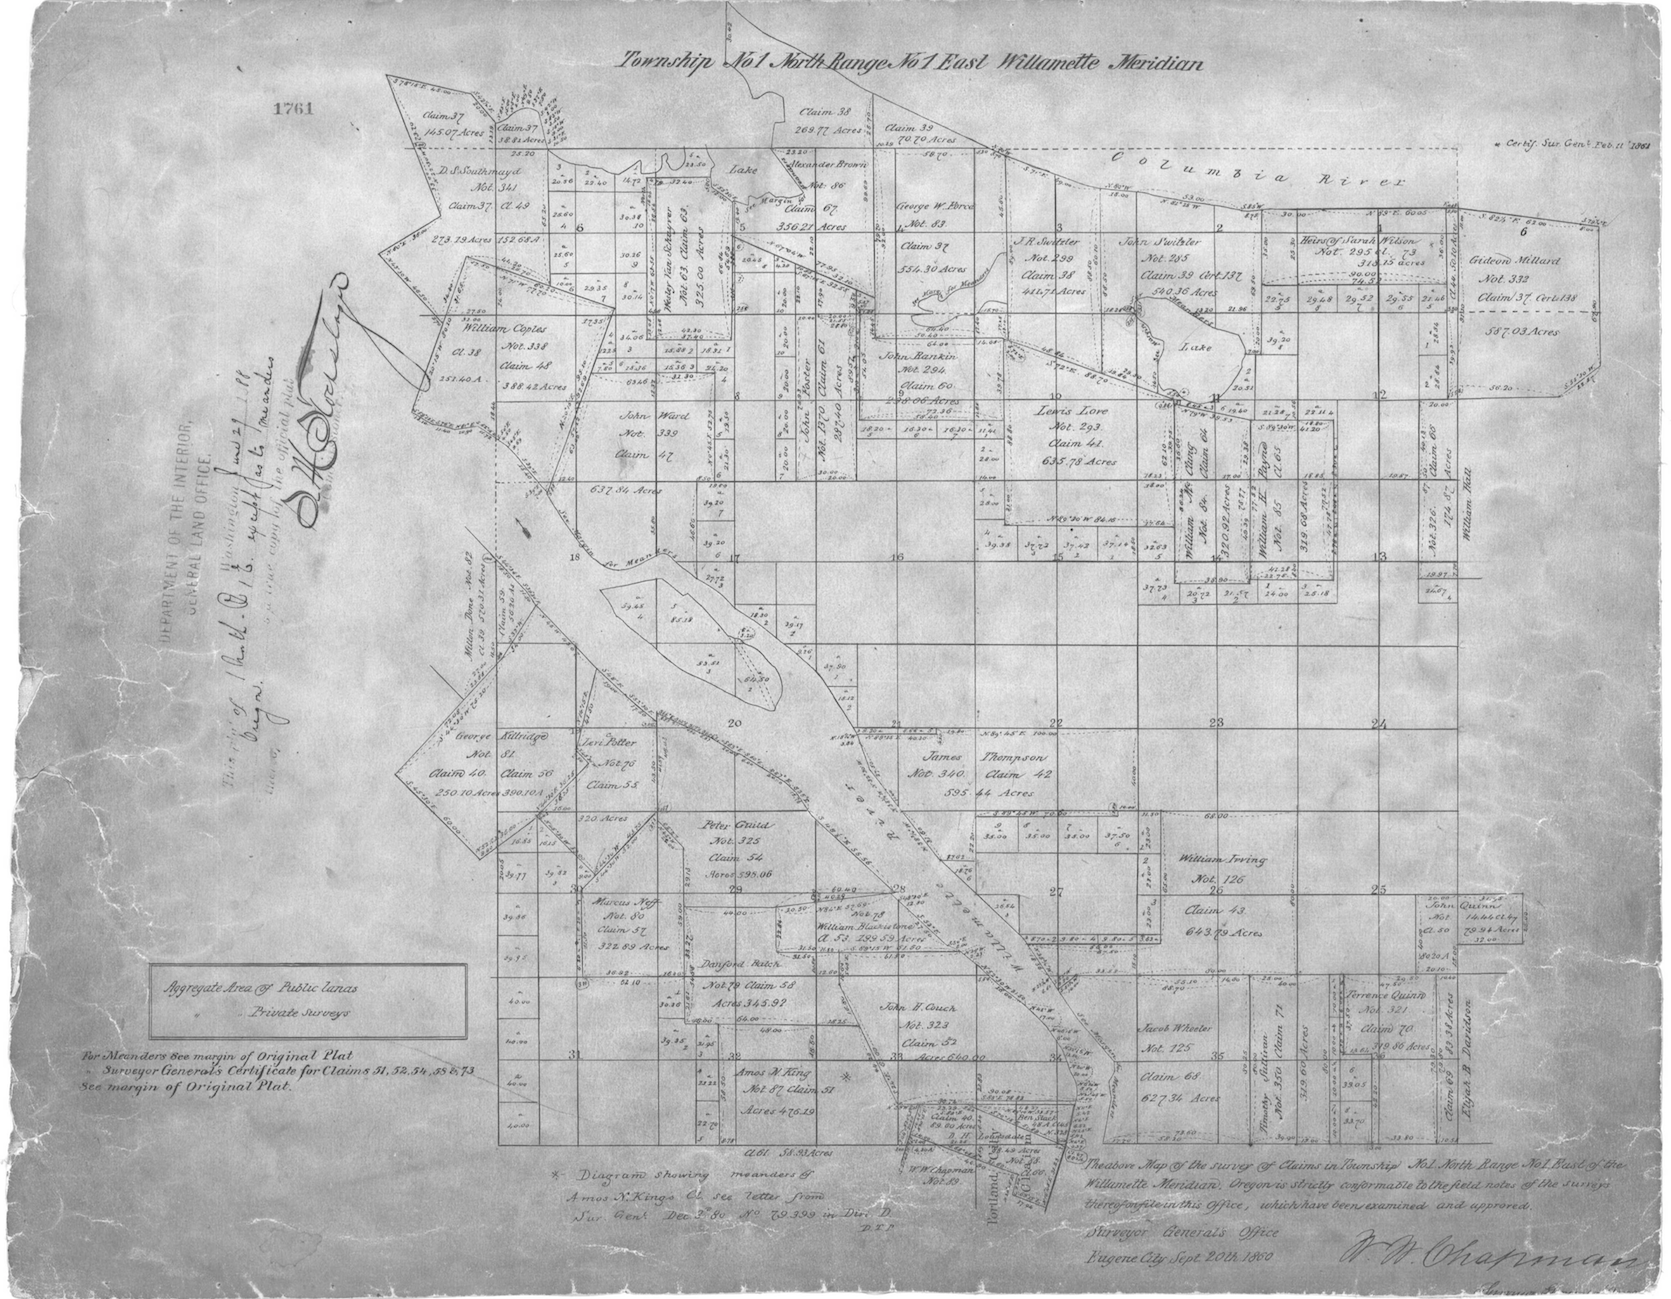
\includegraphics{images/02_images/image2.png}
\caption{alt\_text}
\end{figure}

\url{https://drive.google.com/file/d/1TISCAUaStTYOVqZS58E5ao4AFFOkmzSl}

Remember that links in the captions below pictures and photos generally point to a larger and/or higher resolution version elsewhere on the web. On the map it says, in the lower right hand corner,

\begin{verbatim}
_The above Map of the Survey of Claims in the Township No1 North Range No1 East of the Willamette Meridian, Oregon, is strictly conformable to the field notes of the surveys thereof in file at this office, which have been examined and approved._


_Surveyor General’s Office, Eugene City, September 20th 1860_
\end{verbatim}

The township and range terminology will be discussed later in this introductory chapter, in the section on the Public Land Survey System.

\hypertarget{our-discussion}{%
\section{Our Discussion}\label{our-discussion}}

Each of our homestead chapters is divided into two parts. In the first part I discuss the land, how it was obtained, partitioned, and sold. In the second part I discuss the biographical information I have on the settlers who claimed the land and obtained the patents from the US government. The order of the two parts reflects the emphasis in this book on the ownership of the land, the persons are in some sense accidental, no matter how interesting their lives may have been. But sometimes the division between the land dealings and the life are somewhat artificial, because basically what we know about some of the homesteaders is precisely that they homesteaded in what is now the Piedmont neighborhood. And not much more.

How the land changed hands covers a period from the original claim to the point, often some fifty years later, when the final subdivisions were platted and the plats recorded with Multnomah County. Some plats have hundreds of lots, and it is not feasible to find out and document how individual lots were sold by the original sellers, and then later by the various owners along the way. So I stop at the subdivision level, although there are some exceptions because there is land that was not platted, and there are some lots and buildings on the land with historical significance.

Snyder's 1989 book ``\emph{We Claimed This Land: Portland Pioneer Settlers}'' is impressive, because it covers 212 ``pioneers'', defined as persons or families who ``were the first to settle on the land that is now occupied by the city of Portland, Oregon.'' (1989, preface, page v). But 212 biographies in a book of 278 pages implies that some of them will be very short. Especially because some of the pioneers do get a lot of pages. A. P. Dennison, for example, inexplicably gets 22 pages, which is definitely not proportional to his historical importance. Moreover, Snyder concentrates on pioneers associated with the original site of the City of Portland, on the west side of the Willamette, and on the more urban tracts. This makes perfect sense, because information about them is more readily available. Our Piedmont pioneers Evander Howe (10 lines), George Smith (9 lines), and David Ulery (12 lines) are given short shrift, simply because Snyder does not have more information on them. And some of the information is incorrect or imprecise. Captain Lewis Love gets three pages, which is still not much for such a long and eventful life. John Fenstermacher gets a full page, but mostly because of the tabloid aspects of his life and death. Because we only have to consider just four or five pioneers we can dig much deeper, and find more (and more correct) information.

We freely use the words ``pioneers'' and ``settlers'', although both words have plenty of negative connotations these days (Sakai, 2014). The words seem to suggest that the white people who came from the east arrived on virgin land (the terra nullius doctrine), which was waiting to be occupied, utilized, monetarized, and exploited. The alternative interpretation of what took place in the early nineteenth century is, of course, that all that land was invaded and occupied, and the original inhabitants, the ones that did not succumb to the infectious diseases brought by the settlers, were forcibly removed and in many instances killed. As a rule the white settlers seem to have been brave, daring, inventive, hard working, and incredibly resistant to many kinds of adversity. They came to improve their situation, and many who came early succeeded in doing just that. Their improvement was made possible, however, by the racism, exceptionalism, and manifest destiny ideologies promoted by the ruling classes. And we should not forget they were, wittingly or unwittingly, part of a racist and colonialist invasion that resulted in an horrific genocide (Dunbar-Ortiz, 2014)

\hypertarget{land-laws}{%
\section{Land Laws}\label{land-laws}}

There were multiple laws passed by Congress in the eighteenth and nineteenth century on which the various donations and patents are based. Some of them were actually donations, which means the settlers did not have to pay anything for the land, and some were for-pay, although always for very little money.

Because nothing beats looking at the original documents, in the exact language they were written in, I provide links to the actual laws. In the references at the end of the chapter there are links to Wikipedia articles that provide at least some background. If you want to know more about how the United States disposed on its public lands through a whole sequence of homestead type acts, there is the authoritative article by \href{https://drive.google.com/file/d/1TT_lgoh_nI8LSdztGw_claFQYfHje16G}{Bien (1910)}. For an even more extensive discussion of the donations of various types in Oregon (including giveaways to railroads, timber harvesting, or military wagon roads) see the dissertation by \href{https://drive.google.com/file/d/1T8HRj39qobQ_4NkydJpagwnRQvFPAEUB}{Jerry O'Callaghan (1951)}.

\emph{September 27, 1850: An Act to create the Office of Surveyor-General of the Public Lands in Oregon, and to provide for the Survey, and to make Donations to Settiers of the said Public Lands. \url{https://drive.google.com/file/d/1S69AEHN-PuDvYEKimOUQxD4bzhTkTBSd}}

March 3, 1855: \emph{An Act in Addition to certain Acts granting Bounty Land to certain Officers and Soldiers who have been engaged in Military Service of the United States. }\href{https://drive.google.com/file/d/1Ro5Zk00kgc0UpUnpt7aUpvw05e0H0X6b/view}{https://drive.google.com/file/d/1Ro5Zk00kgc0UpUnpt7aUpvw05e0H0X6b}.

May 20, 1862: An Act to secure Homesteads to actual Settlers in the Public Domain. \url{https://drive.google.com/file/d/1S1TuL2j2sMidQAdCahzAFG4hSx27SkhV}

On the map at the beginning of this chapter Lewis Love and John Rankin used the Oregon Donation Land Act of 1850. John Fenstermacher and Evander Howe used the Homestead Act of 1862 (which means they had to pay for their land). George Smith, Robert Maxey, and David Ulery used the Military Bounty Act of 1855. In all three cases, however, they were not the ones doing the actual military service. By informal and and by now unknowable transactions they made the original military men sign over their patents, undoubtedly for a pittance.

The Oregon Donation Land Act of 1850 deserves some additional attention, because it is specific to our region. The \href{https://drive.google.com/file/d/0B94Urj3OjM7BcWhIYmUtV0htcms}{Genealogical Forum of Oregon (2014)} has a nice brochure, with the essential facts. Also quite readable is the page on the act of the\href{https://oregonhistoryproject.org/articles/historical-records/oregon-land-donation-claim-notification/\#.WriRZS-ZPDY}{Oregon History Project (2018)}.

\hypertarget{public-land-survey-system}{%
\section{Public Land Survey System}\label{public-land-survey-system}}

The \_Rectangular Survey System** **\_was created by the Land Ordinance of 1785. It covers the United States with squares of 6 by 6 miles. It then introduces a local coordinate system by designating a vertical lines (meridian) and horizontal line (base line). In our case the vertical line is the Willamette Meridian, running through the hills west of Portland, and the horizontal line is the Willamette base line, along Base Line Street (now Stark Street). The two intersect at the \href{https://en.wikipedia.org/wiki/Willamette_Stone}{Willamette Stone}. This local coordinate system allows one to code the squares, indicating how many squares east or west of the meridian, and how many squares north or south of the base line they are. The figure below, taken from page 25 of the \href{https://www.blm.gov/or/landsrealty/glo200/files/glo-book.pdf}{excellent e-book by Vaughan (2014)}, show both meridian and base line.

\begin{figure}
\centering
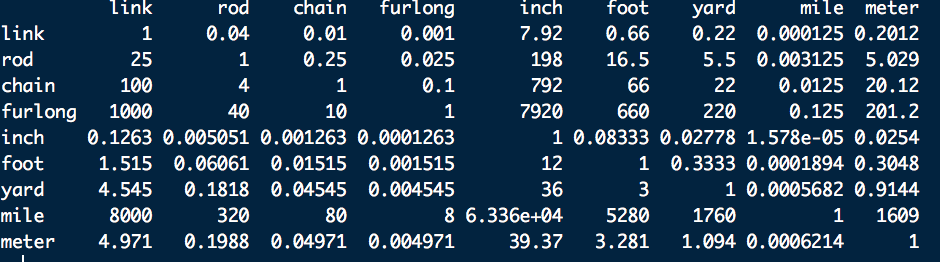
\includegraphics{images/02_images/image3.png}
\caption{alt\_text}
\end{figure}

On the map at the beginning of this chapter you see modern Piedmont in the red boundaries. The black squares are sections 9, 10, 15, and 16 of Township 1 North, Range 1 East (T 1N R 1E), i.e.~the first square north of the baseline and east of the meridian.

A township in PLSS is six by six miles, with 36 sections. Thus T 1N R 1E covers most of Portland. A black section is a square mile, or 640 acres, and the four quarters of a section (NE, SE, SW, NW) are each 160 acres. The following figure, from page 28, of \href{https://www.blm.gov/or/landsrealty/glo200/files/glo-book.pdf}{Vaughan (2014)}, illustrates the basics.

\begin{figure}
\centering
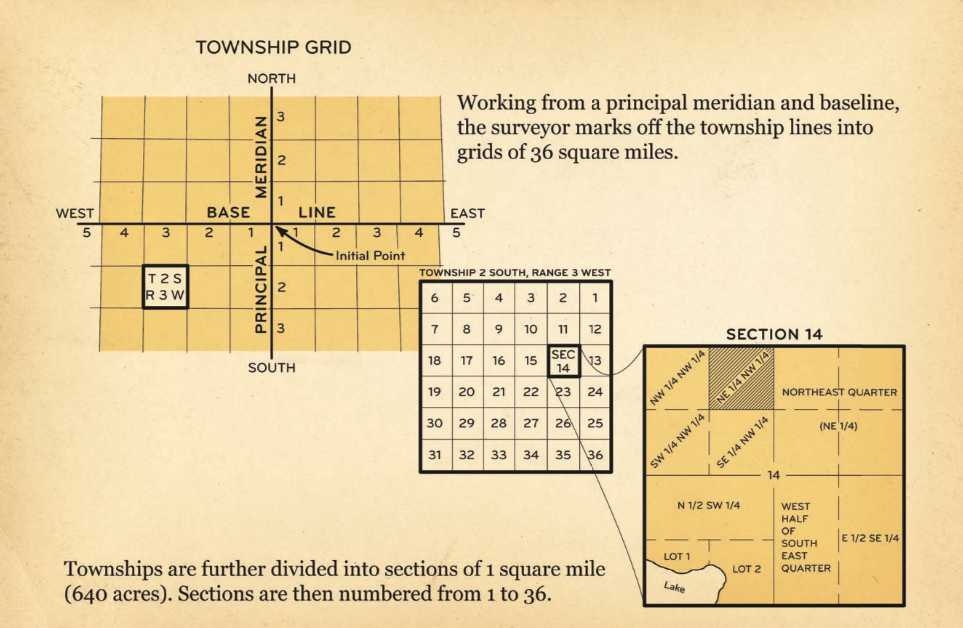
\includegraphics{images/02_images/image4.png}
\caption{alt\_text}
\end{figure}

The rectangular system is used throughout to locate parcels of land, where basically each of the townships provides another even more local coordinate system. We can now say, for example, that a piece of land in the figure above is the SE ¼ of the NW quadrant of Section 14 in township 4 south of range 3 west. Even more importantly, parcels of land, especially in the homestead period, are often defined as sections or quarters of the system, and as a consequence roads often align with boundaries of quarters as well.

\hypertarget{section}{%
\section{}\label{section}}

\hypertarget{surveyors-lengths}{%
\section{Surveyors Lengths}\label{surveyors-lengths}}

In many of the deeds from the nineteenth century parcels of land are described in the language of surveyors, and the boundaries are described in the units of length used by surveyors around that time. Since these units may be unfamiliar to modern readers, I briefly summarize definitions of the most common ones, and show how to translate them into feet and even meters.

\begin{verbatim}
_The name **furlong** derives from the [Old English](https://en.wikipedia.org/wiki/Old_English_language) words furh (furrow) and lang (long). Dating back at least to early [Anglo-Saxon](https://en.wikipedia.org/wiki/Anglo-Saxon) times, it originally referred to the length of the furrow in one [acre](https://en.wikipedia.org/wiki/Acre) of a ploughed [open field](https://en.wikipedia.org/wiki/Open-field_system) (a medieval communal field which was divided into strips). _


_A **chain** is a [unit](https://en.wikipedia.org/wiki/Units_of_measurement) of [length](https://en.wikipedia.org/wiki/Length) that measures 66 [feet](https://en.wikipedia.org/wiki/Foot_(unit)), 22 [yards](https://en.wikipedia.org/wiki/Yard_(unit_of_length)), 100 [links](https://en.wikipedia.org/wiki/Link_(unit)),<sup> </sup>or 4 [rods](https://en.wikipedia.org/wiki/Rod_(unit)) (20.1168 [m](https://en.wikipedia.org/wiki/Metre)). There are 10 chains in a [furlong](https://en.wikipedia.org/wiki/Furlong), and 80 chains in one [statute mile](https://en.wikipedia.org/wiki/Statute_mile). An [acre](https://en.wikipedia.org/wiki/Acre) is the area of 10 square chains (that is, an area of one chain by one furlong). _


_The **rod** or perch or pole is a [surveyor’s](https://en.wikipedia.org/wiki/Surveying) tool<sup> </sup>and unit of [length](https://en.wikipedia.org/wiki/Length) equal to ​5 <sup>1</sup>⁄<sub>2</sub> [yards](https://en.wikipedia.org/wiki/Yard), 16​<sup>1</sup>⁄<sub>2</sub> [feet](https://en.wikipedia.org/wiki/Foot_(length)), ​<sup>1</sup>⁄<sub>320</sub> of a [statute mile](https://en.wikipedia.org/wiki/Statute_mile) or one-fourth of a [surveyor's chain](https://en.wikipedia.org/wiki/Chain_(unit)) and 5.0292 [meters](https://en.wikipedia.org/wiki/Meter). The rod is useful as a unit of length because whole number multiples of it can form one [acre](https://en.wikipedia.org/wiki/Acre) of square measure. _


_The **link** (usually abbreviated as "l.", "li." or "lnk."), sometimes called a **Gunter’s link**, is a [unit](https://en.wikipedia.org/wiki/Physical_unit) of [length](https://en.wikipedia.org/wiki/Length) formerly used in many English-speaking countries. A link is exactly ​<sup>66</sup>⁄<sub>100</sub> of a [foot](https://en.wikipedia.org/wiki/Foot_(unit)), or exactly 7.92 [inches](https://en.wikipedia.org/wiki/Inch) or 20.1168 cm.The unit is based on [Gunter's chain](https://en.wikipedia.org/wiki/Gunter%27s_chain), a metal [chain](https://en.wikipedia.org/wiki/Chain_(unit)) 66 feet long with 100 links, that was formerly used in land [surveying](https://en.wikipedia.org/wiki/Surveying)._
\end{verbatim}

Here is a table to convert links/chains/rods/furlongs to inches/feet/yards/miles and ultimately, for those of us who finally emerged from the middle ages, to meters.

\begin{figure}
\centering
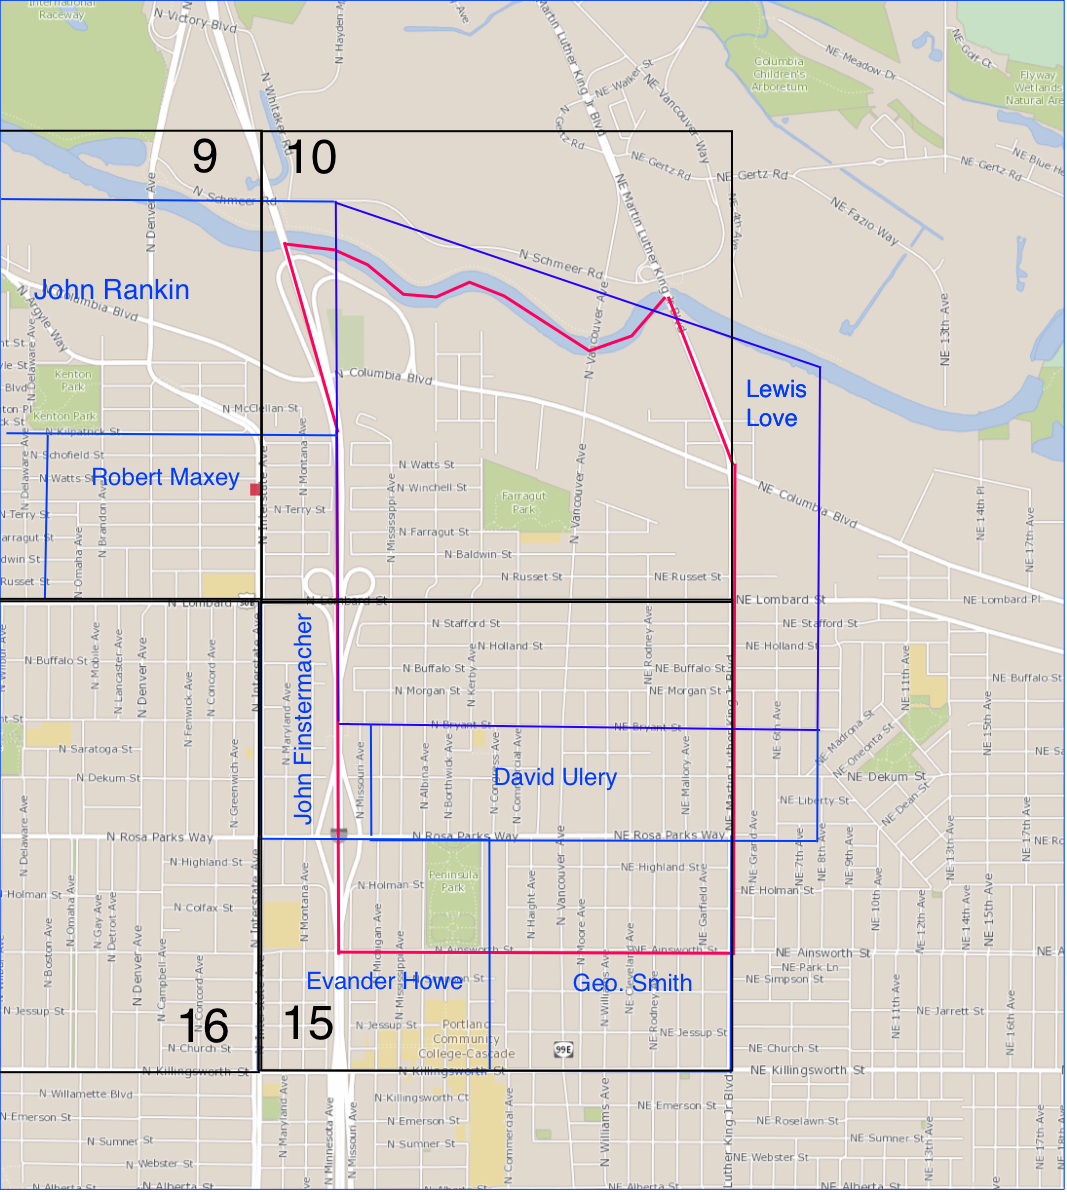
\includegraphics{images/02_images/image5.png}
\caption{alt\_text}
\end{figure}

\hypertarget{deeds-and-patents}{%
\section{Deeds and Patents}\label{deeds-and-patents}}

This book contains excerpts from, transcripts of, and links to hundreds of deeds. There are many types of deeds, which are used to register the transfer of real property. There are hundreds of introductions to deeds and types of ownership of real property of the web. A good example is \href{https://www.americanbar.org/newsletter/publications/law_trends_news_practice_area_e_newsletter_home/2011_summer/real_property_interests_deeds.html}{American Bar Association (2011)}. I only give a brief summary of the types we will encounter in this book.

A \emph{general warranty deed} guarantees that the grantor has clear title, and that no other parties retain an interest in the property. It usually includes various covenants, in particular that the grantor is responsible if it is discovered the title is not clear and third parties makes claims to the property.

A\_ quitclaim deed\_ transfers any interest in the real property that the grantee has to the grantor, without any guarantee that the grantee actually has title to or ownership of the property. Thus the rights of the grantor in the property are transferred to the grantee, provided that the grantor actually has these rights, otherwise the quitclaim deed is just a piece of paper.

A \emph{sheriff's deed} is a deed that gives ownership rights in property bought at a sheriff's sale. A sheriff's sale is a sale conducted by a sheriff upon order of a court after a failure to pay a judgment. These days sheriff's deeds are used in foreclosures, in the nineteenth century they were used even more often if owners of real property failed to pay taxes or bills for goods and services. The important thing is that a court order was needed. Old newspapers have pages and pages of pieces of real estate sold at sheriff's sales, mostly because of delinquent property taxes.

For US land donations and cash transactions under the homestead law we include and transcribe (in as far as they are readable) a copy of the patent and the corresponding deed. For later transfers of real property we include copies, or links to copies, of all deeds we could find. For this chapter we follow the title chain from the US to the homesteader, and then from the homesteader to all next-stage buyers, until the whole homestead is divided up and sold, and we arrive at the subdivision plats, which eventually all will have their separate chapters in this book.

As usual, links to deeds are included, and some deeds, or parts of deeds, are transcribed in the text. Because of the nineteenth century longhand, and because of the quality of the copies and microfilm, it is sometimes impossible to read part of the deed. Also, deeds are to a large extent written in legal language, portions of which are almost the same for all deeds in a certain period. In some cases we skip the boiler plate and only transcribe the variable portions. Finally, we do not transcribe the notarization of the deed, although that is typically included in the linked file.

\hypertarget{plats}{%
\section{Plats}\label{plats}}

\hypertarget{references-2}{%
\section{References}\label{references-2}}

Wikipedia: \emph{Public Land Survey System}

\url{https://en.wikipedia.org/wiki/Public_Land_Survey_System}

Wikipedia: \emph{Link (unit) }

\url{https://en.wikipedia.org/wiki/Link_(unit)}

Wikipedia: \emph{Rod (unit) }

\url{https://en.wikipedia.org/wiki/Rod_(unit)}

Wikipedia: \emph{Chain (unit) }

\url{https://en.wikipedia.org/wiki/Chain_(unit)}

Wikipedia: \emph{Furlong }

\url{https://en.wikipedia.org/wiki/Furlong}

Wikipedia: \emph{Donation Land Claim Act}

\url{https://en.wikipedia.org/wiki/Donation_Land_Claim_Act}

Wikipedia: \emph{Homestead Acts }

\url{https://en.wikipedia.org/wiki/Homestead_Acts}

American Bar Association (2011): \emph{Understanding Real Property Interests and Deeds. }\url{https://www.americanbar.org/newsletter/publications/law_trends_news_practice_area_e_newsletter_home/2011_summer/real_property_interests_deeds.html}

Champ Clark Vaughan (2014): \emph{A History of the United States General Land Office in Oregon.}

\url{https://www.blm.gov/or/landsrealty/glo200/files/glo-book.pdf}

Jerry A. O'Callaghan (1951): \_The Disposition of the Public Domain in Oregon. \_Doctoral Dissertation, Stanford. \url{https://drive.google.com/file/d/1T8HRj39qobQ_4NkydJpagwnRQvFPAEUB}

Roxanne Dunbar-Ortiz (2014): \emph{An Indigenous Peoples' History of the United States.}

Beacon Press, Boston, Massachusetts.

Eugene F. Snyder (1989): \emph{We Claimed this Land. Portland's Pioneer Settlers.}

Binfort \& Mort Publishing, Portland, Oregon

Lorenzo Veracini (2010): \emph{Settler Colonialism. A Theoretical Overview.}

Palgrave MacMillan, New York, NY

Walter L. Hixson (2013): \emph{American Settler Colonialism}

Palgrave MacMillan, New York, NY

J. Sakai (2014): \emph{Settlers. The Mythology of the White Proletariat from Mayflower to Modern.}

Kersplebedeb Publishing and Distribution, Montreal, Quebec

Morris Bien (1910): \emph{The Public Lands of the United States.} The North American Review, 192, 387-402 \href{https://drive.google.com/file/d/1TT_lgoh_nI8LSdztGw_claFQYfHje16G/view}{https://drive.google.com/file/d/1TT\_lgoh\_nI8LSdztGw\_claFQYfHje16G}

Genealogical Forum of Oregon (2014): Oregon Donation Land Claims. \url{https://drive.google.com/file/d/0B94Urj3OjM7BcWhIYmUtV0htcms}

Oregon History Project (2018): \emph{Oregon Land Donation Claim Notification}

\url{https://oregonhistoryproject.org/articles/historical-records/oregon-land-donation-claim-notification/\#.WriRZS-ZPDY}

\hypertarget{references-3}{%
\chapter{References}\label{references-3}}

\end{document}
